\documentclass[12pt,a4paper,titlepage]{article}
\usepackage{fullpage}
\usepackage{hyperref}
\usepackage[pdftex]{graphicx}
\bibliographystyle{plain}
\newcommand{\HRule}{\rule{\linewidth}{0.5mm}}
\usepackage{url}
\usepackage{amsmath}
\usepackage{enumitem}
\usepackage{float}
\usepackage{graphicx}
\usepackage{caption}
\usepackage{subcaption}
\usepackage{tabularx}
\usepackage[nottoc]{tocbibind}
\setlength{\parindent}{0.0in}
\setlength{\parskip}{0.1in}
\begin{document}

\begin{titlepage}
    \let\footnotesize\small
    \let\footnoterule\relax
    \let \footnote \thanks
    \setcounter{footnote}{0}
    \begin{center}
      \setlength{\parskip}{0pt}
       {\large School Of Electronics and Computer Science \par}
      {\large Faculty of Physical and Applied Sciences \par}
      {\large University of Southampton \par}
      \vspace{29mm}
      {\large Argyris Zardilis \par}	
	\vspace{4mm}
      \large \today
	\vspace{13mm}
        \center
        {\Large \bf Tool for parameter inference in dynamic biological systems \par}
        \vspace{60mm}
      {\large Project Supervisor: Dr. Srinandan Dasmahapatra \par }
      {\large Second Examiner: Dr. Markus Brede \par}
      \vspace{12mm}
        {\large A progress report submitted for the award of }\\
      {\large BSc Computer Science }
    \end{center}
    \vfil\null
  \end{titlepage}
\begin{abstract}
Recent advances in experimental technology have given us detailed and comprehensive information on networks of biological interactions governing various functions of living organisms. This had led to an increase in the use of theoretical mathematical models to describe dynamic biological systems which has in turn led to an increasing need for computational tools to assist in the process of constructing these models and estimating their parameters from available experimental data. Although there is a rich literature on parameter estimation using a number of different techniques, very few attempts have been made to systematically attack the parameter estimation problem for these kinds of systems. From those, almost all of them attempt a mere reproduction of experimental data, disregarding important properties of those systems like their qualitative features and the effect of global system dynamics. 

In this study a computational tool has been produced tackling the parameter estimation problem in dynamic biological systems using different techniques and its success has been tested with real world models. Further to that, an attempt has been made to uncover the link and interplay between the practical considerations of the parameter inference process and the more theoretical tools of sensitivity and bifurcation analysis and therefore consequently to systems dynamics which are captured and understood through these. 
\end{abstract}
\tableofcontents
\newpage
\section{Introduction}
Cells of living organisms contain thousands of networks of biochemical interactions that perform their functions. Despite being, at the molecular level, subject to thermal noise and the random tinkering of evolutionary events they are able to perform their functions almost always without error and with remarkable consistency. The apparent high complexity of such networks has been perhaps one of the reasons that the main bulk of biological research has been focused on understanding the details of individual components instead of a systems-level understanding of their interactions. So in a way Biology did not follow the route of other natural sciences, like Physics for example, to try and find simplifying and general principles and laws that govern the behaviour of the natural systems occurring in living organisms using the theoretical framework of Mathematics. It might be because the general consensus was that living organisms are so complex and their behaviour is so highly stochastic at the molecular level that one will not be able to find these laws and express them using a rigorous language like Mathematics as used for inanimate objects. 

However recent advances in experimental technology like microarray experiments which enabled us to get the expression levels of a big number of genes at different time points have given us for the first time such detailed and comprehensive information on cellular processes.  Although the structure of such interactions has been assembled from the effects of many random evolutionary events over time, with this new volume of information we  are able to find common reoccurring network structures which evolution keeps turning to because exactly they are the ones that survive with their robustness. This leads us to think that they are common design principles behind these common network motifs that drive them so the goal of finding generalising and simplifying principles and gain systems level understanding through a theoretical framework inside the apparent complexity is revisited recently shifting some of the attention of biological research from experimentation to more theoretical work\cite{alon2007introduction}. Commonly occurring motifs (network structures) include switches, buzzers, blinkers\cite{tyson2003sniffers}, the inspiration for the decomposition and naming also coming from their resemblance to electronic-like components.

These common network motifs can then be assembled and be parts of larger networks of interactions that perform more complicated functions.  Such networks that their network structure is though to be well understood and have been the subject of much study both experimentally but even more theoretically include circadian oscillators and metabolic pathways\cite{bass2010circadian, sahar2012regulation, mirsky2009model}. As their name suggests one of the main properties of such networks of interactions is their structure, what are the interacting components and which one acts on what. The traditional way to capture this structure is with schematic means with the aid of a diagram an example of which can be seen in Figure \ref{fig:diagram_example}. The components of the network are the nodes of the diagram with their differences highlighted with the use of different shapes or colours while the interactions are the edges differentiated by their ends; in the example the flat end signifies repression while the arrow signifies activation. Several attempts to standardise these diagrams in the example of circuit diagrams in electronics (Molecular Interaction Maps\cite{kohn2006molecular}) have not been widely adopted so they still vary considerably.
\begin{figure}
\centering
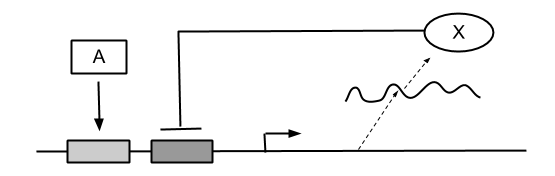
\includegraphics[width=0.5\linewidth]{neg_autoregulation}
\caption{Negative
autoregulation (Dh5a þ pZSp21tetR-egfp4): the tet pro-
moter controls the production of its repressor, TetR
fused to GFP. The TetR – GFP fusion protein represses its
own promoter\cite{rosenfeld2002negative}
}
\label{fig:diagram_example}
\end{figure}

The network structure, though important, is only one of the properties that help us get insight into the workings of these systems. Another essential property which becomes even more apparent as the diagrams and networks grow in size is the systems dynamics. The diagrammatic way of describing the systems is very poor in that sense as it does not capture the dynamic properties that these systems exhibit\cite{kitano2002computational}. The natural way to capture the dynamic behaviour of systems that is being used throughout science is with differential equations. That way we can use a more theoretical and well researched framework of Mathematics and of dynamical systems in particular  to talk about these systems and borrow tools from it that aid the analysis process and give us greater insight to eventually build a systems-level understanding of complex biological systems. The we can ask more complicated and interesting questions like: what are the control mechanisms that drive these systems? how does one part affect others? which parts provide the stability and robustness to the system? How will the system behave in the future with the same or varying conditions? The diagrams which offer the static structure provide very little knowledge and surely cannot answer these questions.

Systems can be thought of as stochastic processes as they are subject to molecular noise and various fluctuations in their interactions. Therefore they can be expressed as stochastic differential equations or their evolution can be simulated with the Gillespie algorithm or more recent variants.\cite{}. However the effects of these fluctuations are only considerable when the number of molecules of the reactants is very small so more oftenly the average case is considered and the systems are expressed as deterministic Ordinary Differential Equations(ODEs). These describe the evolution in the concentrations of components of the systems(variables) over time. These equations are translations of the diagrams and the duality of the representation can be seen through an example of translating the diagram in Figure\ref{fig:diagram_example} to equations.  


This is a simple network motif of a switch blah blah 
\subsection{Dynamical Systems}

\section{Background}

\section{Work}

\subsection{Methods}

\subsection{Results}

\section{Discussion and Future Work}

\newpage
\bibliography{report}
\appendix
\section{Time Management}
\section{Critical Evaluation}
\end{document}